\chapter{Technologieën}
In dit hoofdstuk wordt er gekeken naar technologieën die eventueel toepasbaar zijn op het ontwikkelproces van de nieuwe editor. Eerst zullen de huidige gebruikte technologieën op een rijtje worden gezet. Hierna zal er gekeken worden naar de toekomst van de editors. Tenslotte zal het probleem in kaart worden gebracht waarop eventuele oplossingen zullen worden geadviseerd.

\section{Wat wordt er verstaan onder ‘technology stack’}
Onder een ‘technology stack’ (of ‘tech stack’) verstaan we de onderliggende bouwblokken waarop de desbetreffende applicatie gebouwd is. Deze bouwblokken bestaan uit onder andere frameworks, libraries, programmeertalen, softwareproducten en eventuele tooling\cite{BlogTechStack}.

\section{Waarom is dit belangrijk?}
Het is erg belangrijk om de tech stack in kaart te brengen omdat er elementaire informatie uit te halen is. De tech stack geeft inzicht in hoe het huidige product in elkaar steekt en eventuele consequenties wanneer er componenten in de stack aangepast worden. Dit is noodzakelijk voor het maken van een nieuwe editor die geïntegreerd moeten worden in een al bestaande tech stack. Door deze stap te nemen wordt er goed gekeken naar hoe de nieuwe editor in het totaal plaatje zou kunnen passen. Zo kan het voor komen dat er bepaalde software wordt gebruikt die nauw samenwerkt met de huidige editors. Dit heeft als gevolg dat de nieuwe editors deze samenwerking moeten ondersteunen.

\section{Huidige ontwikkelomgeving}
Om de ontwikkeling van narrative games te ondersteunen heeft het bedrijf een ontwikkelomgeving opgezet. Het doel van deze omgeving is om het ontwikkelingsproces inzichtelijk te maken voor verschillende disciplines en overtollig werk, zoals het opzetten van een nieuw project, te vermijden door een leeg raamwerk aan te bieden. Dit raamwerk bevat templates (het NGT), editors en programma’s om de efficiëntie en collaboratie tijdens het ontwikkelproces te bevorderen.

De ontwikkelomgeving voor narrative games heeft een onderliggende tech stack die bestaat uit verschillende programmeertalen, libraries, frameworks, Integrated development environments (IDE’s) en externe applicaties. Stackshare.io\footnote{https://stackshare.io/} een website waar stacks van (bekende) bedrijven kunnen worden ingezien, deelt deze op in de volgende lagen\cite{StackShareCategories}:

\begin{itemize}
    \item \textbf{Application and Data}, dit betreft onder andere programmeertalen, frameworks \& libraries.
    \item \textbf{Utilities}, hieronder vallen analytics en eventuele hulpmiddelen.
    \item \textbf{DevOps}, gaat over de build, test, deploy processen en het monitoren van het product.
    \item \textbf{Business Tools}, omvangt bestaande oplossingen voor samenwerking en marketing.
\end{itemize}

De onderliggende tech stack die de ontwikkelomgeving van narrative games ondersteund kan uiteen worden gezet volgens deze lagen. Hierdoor kan inzicht worden verkregen in hoe de huidige ontwikkelomgeving in elkaar steekt. Het bedrijf beschrijft de narrative game: ‘Mission Zhobia: Winning the Peace’ als een typische narrative game. Dit spel beschikt over de volgende tech stack:


\begin{table}[htb]
    \centering
    \begin{tabular}{ | l | l | }
        \hline
        \multicolumn{2}{|c|}{Narrative game - Technology stack} \\
        \hline
        \multicolumn{2}{|c|}{Application and Data} \\
        \hline
        \&ranj JavaScript software library & \tabitem Javascript(ECMAScript5) \\
        & \tabitem CreateJS suite \\
        Narrative game template & \tabitem Javascript(ECMAScript5) \\
        & \tabitem CreateJS suite \\
        & \tabitem SomaJS \\
        \&ranj ActionScript3 software library\footnote{Bestaat uit 3 ActionScript3 libraries gemaakt door \&ranj, maar heeft één verzamelnaam} & \tabitem ActionScript3 \\
        Story- \& dialog editor & \tabitem ActionScript3 \\
        & Apache Flex \\
        & Flex wires \\
        \hline
        \multicolumn{2}{|c|}{Utilities} \\
        \hline
        Analytics & \tabitem Google Analytics \\
        \hline
        \multicolumn{2}{|c|}{DevOps} \\
        \hline
        Source control & \tabitem Beanstalk \\
        & \tabitem SourceTree \\
        Deployment & \tabitem Jenkins \\
        & \tabitem SourceTree \\
        IDE'S & \tabitem Adobe Flashbuilder\footnote{Bouwt ook de editors} \\
        & Netbeans \\
        Monitoring & \tabitem Pingdom \\
        \hline
        \multicolumn{2}{|c|}{Business Tools} \\
        \hline
        Collaboratie & \tabitem Trello \\
        & \tabitem G Suite \\
        & \tabitem Slack \\
        Documentatie & \tabitem \&ranj wiki \\
        \hline
    \end{tabular}
    \caption{Huidige technology stack}
\end{table}

Dit onderzoek betreft het opzetten van (flexibele) editors, daarom is het essentieel om de relatie tussen de huidige editors en de andere componenten binnen de ‘Application and Data’ laag in kaart te brengen. Hier kunnen eventuele risico’s/ consequenties naar aanleiding van veranderingen worden uitgelicht. Het is van belang dat de nieuwe editor goed aansluit bij de rest van de stack, zodat er onderbouwd advies op het gebied van veranderingen in de tech stack uitgebracht kan worden. De relaties tussen de componenten in de ‘Application and Data’ laag zijn weergeven in \autoref{fig:editorrelations}.

\begin{figure}[htb]
    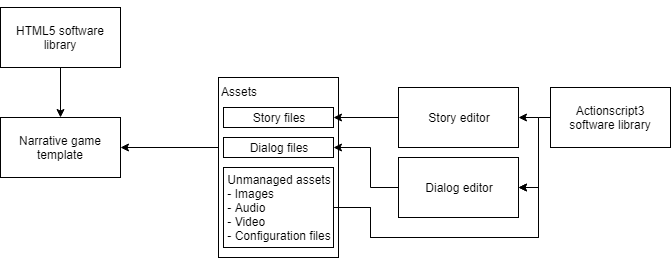
\includegraphics[width=\textwidth,height=\textheight,keepaspectratio]{StoryDialogEditorRelations}
    \caption{Story- en dialog editor relaties}
    \label{fig:editorrelations}
    \centering
\end{figure}

\section{Toekomst van de editors}
De toekomst van de editors zal, zoals in de inleiding beschreven, bestaan uit een web omgeving waarin meerdere personen tegelijk kunnen werken (collaborative editing). Hierin worden aanpassingen direct getoond aan teamleden wat het mogelijk maakt om met elkaar samen te werken aan dezelfde bestanden. Deze feature wordt nog interessanter wanneer klanten bij het ontwikkelproces betrokken worden. Zij zouden dan directe feedback of zelfs aanpassingen kunnen doen aan de game content. Het bedrijf geeft aan dat ze hier in de toekomst naar toe gaan werken, maar dat er meer onderzoek en resources nodig zijn om dit mogelijk te maken.

Hoewel dit vraagstuk niet in dit onderzoek past kan er wel rekening mee worden gehouden. Ook al zal het bedrijf voorlopig gebruik maken van een desktopapplicatie, moet er wel een blik op de toekomst geworpen worden. Bij het opzetten van een nieuwe editor vindt \organisation{} toekomstgerichtheid een belangrijk aspect; het bedrijf wil dan ook niet opnieuw een hele editor opzetten. Bij de keuzes die invloed hebben op de tech stack zal hier dan ook op worden gelet.

\section{Probleem}
Beschikken over een stabiele en toekomstig gerichte tech stack is cruciaal voor een succesvol product. De tech stack heeft een directe invloed op de toegankelijkheid, schaalbaarheid en toekomstgerichtheid van de toekomstige editor. 

\subsection{Onzekerheid in de toekomst}
De huidige editors zijn gemaakt in Apache Flex. Dit is een omgeving waarin applicaties gemaakt kunnen worden met de hulp van ActionScript3 om logica te kunnen programmeren en MXML wat het definiëren van lay-outs toelaat in een XML-formaat\cite{WhatIsApacheFlex}. Projecten kunnen gecompileerd worden naar SWF-bestanden die kunnen worden uitgevoerd in een Flash- of Air run time. Vorig jaar, 25 juli, liet Adobe in een blog post weten dat ze ondersteuning voor Flash gaan beëindigen in 2020\cite{AdobeFlashFuture}. Hiernaast lijken er ook weinig updates plaats te vinden. Volgens de website van Apache Flex was de laatste update op 22 november 2017\cite{ApacheFlex}. Tenslotte werd Flash al eerder in meerdere populaire browsers standaard geblokkeerd vanwege veiligheidsredenen\cite{FlashWillBeBlocked}. Dit gaat tegen het toekomstbeeld van de editors in, het bedrijf wilt toewerken naar een webapplicatie. Verder leidt dit alles naar een onzekere toekomst van Apache Flex.

\subsection{Kleine community}
Het aanbod van libraries, klare oplossingen op veelvoorkomende problemen, is naar verhouding vrij minimaal omdat de community rond Apache Flex en ActionScript3 in vergelijking tot andere ontwikkelomgevingen relatief klein is. In de ‘populaire technologieën’ sectie van de enquête die Stack Overflow jaarlijks afneemt zijn Apache Flex en ActionScript3 niet te vinden\cite{StackOverflowSurvey2018}. Ondanks dat de Apache Flex community wel op Stack Overflow zit\cite{StackOverflowFlexQuestions}. Een kleinere community kan leiden tot minder hulp en een gebrek aan oplossingen voor veel voorkomende problemen. Dit is ook terug te zien aan ‘Flex Wires’, een library die de editors gebruiken om de nodes met lijnen aan elkaar te verbinden. De library is slecht aanpasbaar en biedt weinig functionaliteit. Verbindingen kunnen niet aangepast worden, er verschijnt altijd een grijze kromme lijn. Dit heeft als gevolg dat bepaalde features niet haalbaar zijn in de huidige editors. Hiernaast zitten er fouten in Flex Wires die alleen opgelost kunnen worden in de library zelf. Zo kunnen de verbindingen uit het niks verdwijnen, waardoor niet meer te zien is welke relaties er bestaan tussen nodes.

\subsection{Overtollige libraries}
Zowel de editors als het NGT maken gebruik van de \organisation{} software library welke generieke functionaliteiten en datastructuren bevat (zie \autoref{fig:editorrelations}). Echter moeten er twee libraries onderhouden worden omdat de huidige editors en het NGT geschreven zijn in verschillende programmeertalen. Het implementeren van nieuwe generieke functionaliteiten moet dubbel gedaan worden en de libraries moeten beide up-to-date zijn, omdat het NGT en de editors anders mogelijk niet meer goed samen kunnen werken.